Om een restore point terug te zetten gaan we naar System Properties en kiezen we \textquote{System Restore...}. We kunnen daar het restore point selecteren waar we naar terug willen. De knop \textquote{Scan for affected files} geeft je een overzicht wat er wordt terug gezet.

\begin{minipage}[t]{\linewidth}
\raggedright
\adjustbox{valign=t}{%
   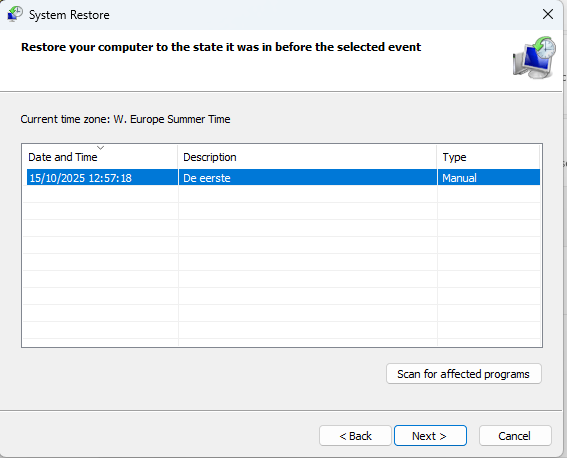
\includegraphics[width=0.75\linewidth]{system_protection-restore.png}%
}
\end{minipage}

Afhankelijk van hoeveel er terug gezet moet worden kan een restore enige tijd duren.

